\begin{figure}[ht] 
 	\centering 
 	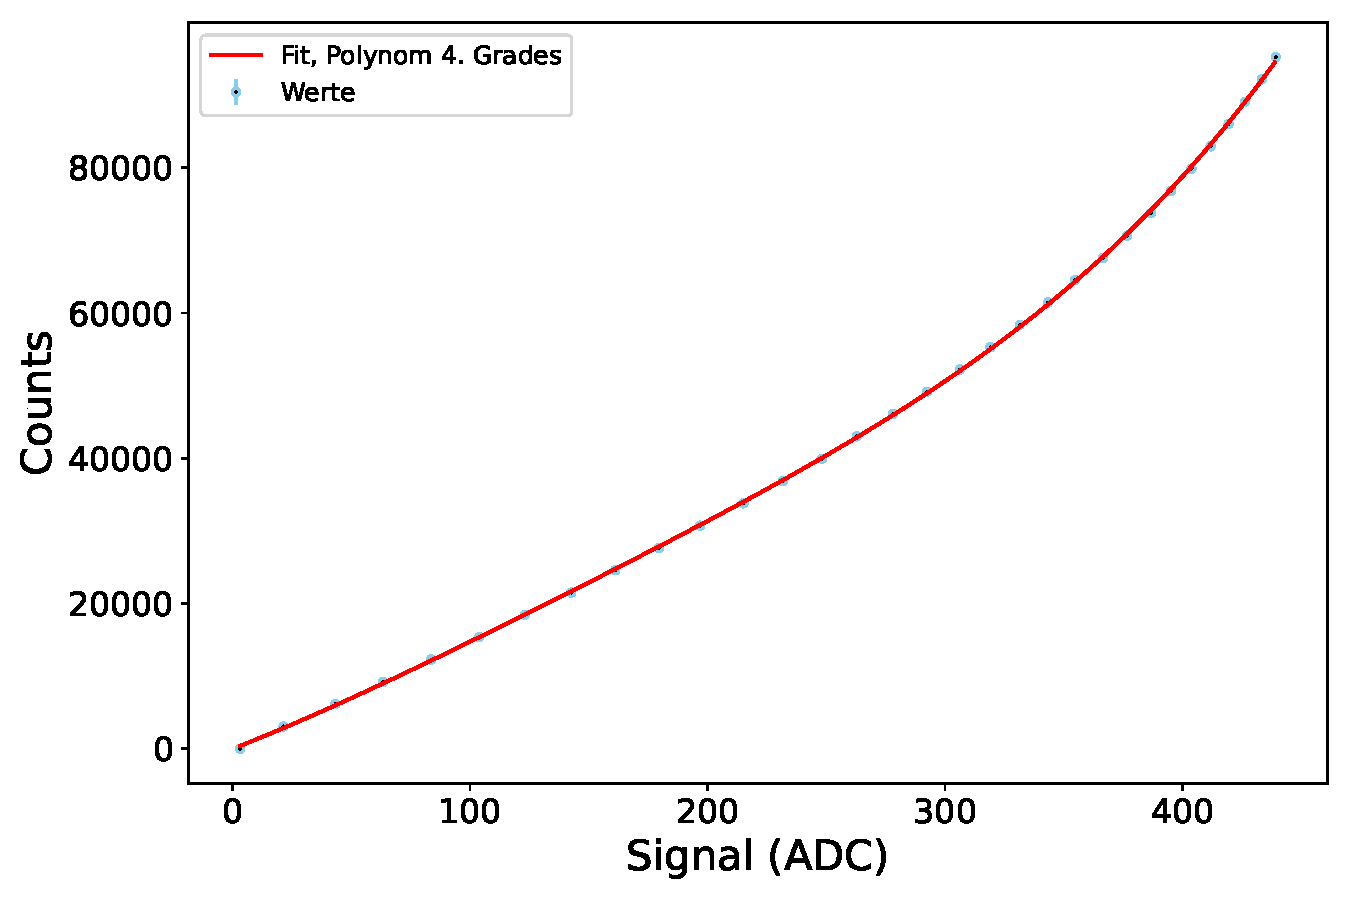
\includegraphics[width= 0.65 \textwidth]{Fits/A3_Cali_Charge_Fit.pdf} 
	\caption{A3_Cali_Charge, Fit} 
 	\label{fig:A3_Cali_Charge, Fit} 
\end{figure}
 \\ 
\begin{table}[ht] 
\centering 
\caption{A3_Cali_Charge, Fit Parameter Tabelle} 
\label{tab:my-table}
\begin{tabular}{|l|c|}
\hline
Parameter Name	&	Wert \\ \hline
a	&	 2.29e-06 \pm  2.35e-07\\ \hline
b	&	-0.0012417 \pm  0.000214\\ \hline
c	&	 0.305 \pm  0.0641\\ \hline
d	&	 127.158 \pm  7.027\\ \hline
e	&	-31.3280 \pm  223.438\\ \hline
\end{tabular} 
\end{table}